% This file was created with tikzplotlib v0.10.1.
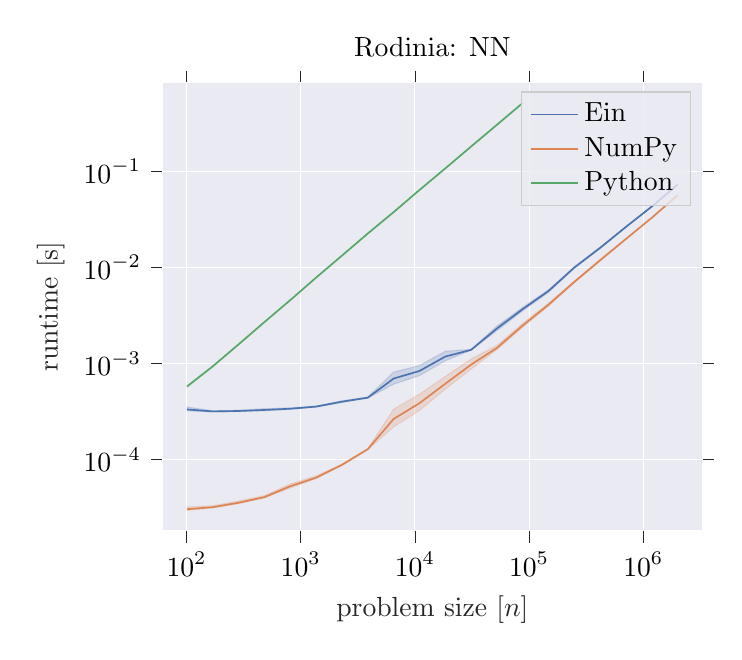
\begin{tikzpicture}

\definecolor{darkslategray38}{RGB}{38,38,38}
\definecolor{lavender234234242}{RGB}{234,234,242}
\definecolor{lightgray204}{RGB}{204,204,204}
\definecolor{mediumseagreen85168104}{RGB}{85,168,104}
\definecolor{peru22113282}{RGB}{221,132,82}
\definecolor{steelblue76114176}{RGB}{76,114,176}

\begin{axis}[
axis background/.style={fill=lavender234234242},
axis line style={white},
legend cell align={left},
legend style={
  fill opacity=0.8,
  draw opacity=1,
  text opacity=1,
  draw=lightgray204,
  fill=lavender234234242
},
log basis x={10},
log basis y={10},
tick align=outside,
title={Rodinia: NN},
x grid style={white},
xlabel=\textcolor{darkslategray38}{problem size \(\displaystyle [n]\)},
xmajorgrids,
xmajorticks=true,
xmin=61.5865594359247, xmax=3279936.43174958,
xmode=log,
xtick style={color=darkslategray38},
xtick={1,10,100,1000,10000,100000,1000000,10000000,100000000},
xticklabels={
  \(\displaystyle {10^{0}}\),
  \(\displaystyle {10^{1}}\),
  \(\displaystyle {10^{2}}\),
  \(\displaystyle {10^{3}}\),
  \(\displaystyle {10^{4}}\),
  \(\displaystyle {10^{5}}\),
  \(\displaystyle {10^{6}}\),
  \(\displaystyle {10^{7}}\),
  \(\displaystyle {10^{8}}\)
},
y grid style={white},
ylabel=\textcolor{darkslategray38}{runtime \(\displaystyle [\mathrm{s}]\)},
ymajorgrids,
ymajorticks=true,
ymin=1.81947944318841e-05, ymax=0.839521688084527,
ymode=log,
ytick style={color=darkslategray38},
ytick={1e-06,1e-05,0.0001,0.001,0.01,0.1,1,10},
yticklabels={
  \(\displaystyle {10^{-6}}\),
  \(\displaystyle {10^{-5}}\),
  \(\displaystyle {10^{-4}}\),
  \(\displaystyle {10^{-3}}\),
  \(\displaystyle {10^{-2}}\),
  \(\displaystyle {10^{-1}}\),
  \(\displaystyle {10^{0}}\),
  \(\displaystyle {10^{1}}\)
}
]
\path [draw=steelblue76114176, fill=steelblue76114176, opacity=0.2]
(axis cs:101,0.000353183350853215)
--(axis cs:101,0.000322000755368208)
--(axis cs:170,0.000314380267118395)
--(axis cs:286,0.000317003530926741)
--(axis cs:481,0.000322697213905485)
--(axis cs:810,0.000334883444993466)
--(axis cs:1364,0.000352830739120691)
--(axis cs:2297,0.000393298693052202)
--(axis cs:3866,0.000437682356459845)
--(axis cs:6508,0.000610060642447934)
--(axis cs:10954,0.000748529692882585)
--(axis cs:18439,0.00107022395513923)
--(axis cs:31037,0.0013778470563193)
--(axis cs:52243,0.00220267150323707)
--(axis cs:87937,0.00354220306126081)
--(axis cs:148018,0.00552566797723557)
--(axis cs:249149,0.00984000897233273)
--(axis cs:419374,0.0157586040781098)
--(axis cs:705902,0.0262687281757098)
--(axis cs:1188194,0.0427564917887139)
--(axis cs:2000000,0.0721616613371225)
--(axis cs:2000000,0.0738775504718173)
--(axis cs:2000000,0.0738775504718173)
--(axis cs:1188194,0.0434651341967401)
--(axis cs:705902,0.0266722735361873)
--(axis cs:419374,0.0162754852996295)
--(axis cs:249149,0.0101439765249415)
--(axis cs:148018,0.00586161805647862)
--(axis cs:87937,0.0038486267659755)
--(axis cs:52243,0.00245423619433495)
--(axis cs:31037,0.00140523523068623)
--(axis cs:18439,0.0013424137828224)
--(axis cs:10954,0.000953390890881565)
--(axis cs:6508,0.000815215431102843)
--(axis cs:3866,0.00044905472001119)
--(axis cs:2297,0.00040965498505102)
--(axis cs:1364,0.000361619109044113)
--(axis cs:810,0.000346027625691931)
--(axis cs:481,0.000339486644388671)
--(axis cs:286,0.000327328193470748)
--(axis cs:170,0.000322710332693532)
--(axis cs:101,0.000353183350853215)
--cycle;

\path [draw=peru22113282, fill=peru22113282, opacity=0.2]
(axis cs:101,3.22559100401596e-05)
--(axis cs:101,2.96449693902489e-05)
--(axis cs:170,3.14934114268439e-05)
--(axis cs:286,3.48214441480291e-05)
--(axis cs:481,4.00659476672678e-05)
--(axis cs:810,5.07766298240826e-05)
--(axis cs:1364,6.35731459038473e-05)
--(axis cs:2297,8.71387222680512e-05)
--(axis cs:3866,0.0001274504644238)
--(axis cs:6508,0.000219516355946705)
--(axis cs:10954,0.00032421837460516)
--(axis cs:18439,0.000541176797972362)
--(axis cs:31037,0.000875860084372431)
--(axis cs:52243,0.00139754218193783)
--(axis cs:87936.9999999999,0.00238507747289486)
--(axis cs:148018,0.00397239848397111)
--(axis cs:249149,0.00693343404896193)
--(axis cs:419374,0.011701289388949)
--(axis cs:705902,0.0196380316798663)
--(axis cs:1188194,0.0327551329863903)
--(axis cs:2000000,0.0563697438910666)
--(axis cs:2000000,0.0567656971331198)
--(axis cs:2000000,0.0567656971331198)
--(axis cs:1188194,0.0330266446635957)
--(axis cs:705902,0.020009598896486)
--(axis cs:419374,0.0121253361396363)
--(axis cs:249149,0.00723793720397841)
--(axis cs:148018,0.00425602114828713)
--(axis cs:87936.9999999999,0.00262417958025749)
--(axis cs:52243,0.00154237070974182)
--(axis cs:31037,0.00111702348559922)
--(axis cs:18439,0.000733776703379504)
--(axis cs:10954,0.000480482764834311)
--(axis cs:6508,0.000334941548718695)
--(axis cs:3866,0.000130604314644266)
--(axis cs:2297,9.00585693711033e-05)
--(axis cs:1364,6.78827531542254e-05)
--(axis cs:810,5.5947379509631e-05)
--(axis cs:481,4.22765473712785e-05)
--(axis cs:286,3.71984245268413e-05)
--(axis cs:170,3.31572100669677e-05)
--(axis cs:101,3.22559100401596e-05)
--cycle;

\path [draw=mediumseagreen85168104, fill=mediumseagreen85168104, opacity=0.2]
(axis cs:101,0.000589457024414009)
--(axis cs:101,0.000568953687788088)
--(axis cs:170,0.000932760601906098)
--(axis cs:286,0.00157676212682705)
--(axis cs:481,0.00269014023387063)
--(axis cs:810,0.00456824403507154)
--(axis cs:1364,0.00781684567576174)
--(axis cs:2297,0.0132332147399879)
--(axis cs:3866,0.0224030687894545)
--(axis cs:6508,0.0375410743138903)
--(axis cs:10954,0.0636976314951003)
--(axis cs:18439,0.106880695886844)
--(axis cs:31037,0.180381141286895)
--(axis cs:52243,0.302955803728834)
--(axis cs:87936.9999999999,0.513305702468478)
--(axis cs:87936.9999999999,0.515261943256742)
--(axis cs:87936.9999999999,0.515261943256742)
--(axis cs:52243,0.306912435547992)
--(axis cs:31037,0.181994994172091)
--(axis cs:18439,0.107544237911094)
--(axis cs:10954,0.0641120078648686)
--(axis cs:6508,0.0377682359528933)
--(axis cs:3866,0.0227212726354391)
--(axis cs:2297,0.0133415728676727)
--(axis cs:1364,0.00787460561231384)
--(axis cs:810,0.00458809586848752)
--(axis cs:481,0.00272029211130062)
--(axis cs:286,0.00159993491855368)
--(axis cs:170,0.000943961562623982)
--(axis cs:101,0.000589457024414009)
--cycle;

\addplot [semithick, steelblue76114176]
table {%
101 0.000333293699804926
170 0.000317854050808819
286 0.000321154150879011
481 0.000329189600597601
810 0.000339143750170479
1364 0.000356783248571446
2297 0.000401624949881807
3866 0.000441795850929338
6508 0.000698466801986797
10954 0.000837535450409632
18439 0.00118185419923975
31037 0.0013890062495193
52243 0.00231618305042502
87937 0.00368823744938709
148018 0.00569290025014197
249149 0.00999016645146185
419374 0.0160098270993331
705902 0.0264645334005763
1188194 0.043052987599367
2000000 0.0728267559284827
};
\addlegendentry{Ein}
\addplot [semithick, peru22113282]
table {%
101 3.05528342139521e-05
170 3.2091806616217e-05
286 3.56759428016795e-05
481 4.08118615742292e-05
810 5.29794457754726e-05
1364 6.50958708510871e-05
2297 8.83896944339121e-05
3866 0.000128688389726388
6508 0.000265278999709473
10954 0.000387513753608334
18439 0.000616376754286184
31037 0.000975915411108311
52243 0.00145488893584056
87936.9999999999 0.00249228061874149
148018 0.00410179624561609
249149 0.00708321676797298
419374 0.0119003698396945
705902 0.0198239321008911
1188194 0.0328866681925195
2000000 0.0565629873357129
};
\addlegendentry{NumPy}
\addplot [semithick, mediumseagreen85168104]
table {%
101 0.000577430156660138
170 0.000938021977295833
286 0.00158729640319589
481 0.00270493801690121
810 0.00457767140090912
1364 0.00784705169005239
2297 0.0132865399300266
3866 0.0225482732543257
6508 0.037647948818945
10954 0.0639124892179613
18439 0.107201755226209
31037 0.181154204295067
52243 0.304895639952628
87936.9999999999 0.514365493283406
};
\addlegendentry{Python}
\end{axis}

\end{tikzpicture}
